

% Since the semantics of permutation problem differs, many dedicated models are designed for specific permutation problems. For example, the EHBSA outperforms than other algorithms on TSP~\citep{tsutsui2002probabilistic}, while the NHBSA is dedicated to the problems with strong relation of absolute positions of indices like QAP. Despite the diversity of semantics, a model can only focus on specific permutation problems. Furthermore, The semantics of permutation is not always clear to the literature. It increases the difficulty to chooses the appropriate model to solve the permutation problems. As a result, existing models can not perfectly capture the core semantics which beyond the capability of existing models. 

% To conquer the difficulty of EDAs on permutation problems, a tool allowing EDAs to adapt itself to the problems is needed. The model adaptation framework should determine which semantic model is the fittest for the problem and acquire the solutions as close as possible to the global optima. To Achieve this, learning techniques are necessary for the model adaptation. Similarly, the model adaptation also faces the some difficulty when choosing model to sample new individual. When the system initials, no prior knowledge about the relation between the problem and the models is given. Through repeated trials within limited NFE, the system has to find out the fittest model for specific problem and manages to yield the solution as close as possible to the result a single model EDA would provide.




\section{Multi-armed Bandit Based Model Adaptation}
At the last attempt, we use the UCB algorithm to choose model. The UCB algorithm is commonly used to solve multi-armed bandit problem. This chapter shows the introduction of UCB and the model adaptation framework.

Ideally, we choose one of the most expressive semantic models for the problem in each generation to reduce NFE. However, without given the semantics of the problem in prior, we can only explore several different semantic models information before fully exploiting the most promising model. Therefore, we use the techniques from the multi-armed bandit problem to balance exploration and exploitation.

\subsection{Multi-armed Bandit Problem}
% Multi-Armed Bandit Algorithms and Empirical Evaluation
A multi-armed bandit (MAB) is like a traditional slot machine but with $K$ levers. When pulled, each lever provides a reward drawn from the distribution associated to that specific lever. The gambler has no prior knowledge of reward distribution of the levers, but through repeated trials, he can focus on the most profitable lever~\citep{Mohri2005, Kuleshov2000}.

The classic MAB problem consists of random variables $X_{i,n}$ for $1\leq i\leq K$ and $n\geq 1$, where each $i$ stands for the index of a gambling machine (\textit{i.e.}, the arm of a bandit). Successive plays of machine $i$ yield rewards $X_{i,1}, X_{i,2},...$ which are independent and identically distributed by unknown law and with unknown expectation. 

For a formal definition, the random variables are independent across the arms and are associated to probability distributions $(D_1, D_2,...,D_k)$ with  expectations $(\mu_1, \mu_2,...,\mu_k)$ and variances $(\sigma_1, \sigma_2,...,\sigma_k)$. Throughout the playing, the distributions are unknown for gambler. The goal for gambler is to collect as much rewards as possible by pulling the armed over many times. At each turn, $t=1,2,...$, the gambler selects an arm, with index $j(t)$ and the times played $n$, and receives a reward $X_{j(t),n}$. The MAB algorithms specify a strategy or a polity by
which the gambler should choose an arm $i$ at each turn. 

%  Asymptotically efficient adaptive allocation rules.
The most popular performance measure for bandit algorithms is the total \textit{expected regret},
defined for any fixed turn $T$ as:
\begin{equation*}
    R_T = T\mu^* - \sum^T_{t=1}{\mu_{j(t)}} \text{,}
\end{equation*}
where $\mu^* = \max_{i=1,...,k}{\mu_i}$ is the expected reward from the best arm.  Thus, the regret is the loss caused by the policy not always playing the best machine. For a large class of pay-off distributions, there is no policy whose regret would grow slower than $O(\ln n)$~\citep{lai1985asymptotically}. For such pay-off distributions, a policy is said to resolve the exploration-exploitation trade-off if its regret growth rate is within a constant factor of the best possible regret rate.


\subsection*{Upper Confidence Bound Algorithms}
% 2002 - Finite-time Analysis of the Multi-armed Bandit Problem
% 2006 - Bandit Based Monte-Carlo Planning
The UCB algorithms have been proposed by~\citep{Auer2002, Auer2002ucb} which are a family of widely used in the MAB problem.  The UCB family was designed as a simpler, more elegant implementation of the idea of optimism in the face of uncertainty, proposed by Lai \& Robbins~\citep{lai1985asymptotically}. An extension of UCB-style algorithms to sequential, tree-based planning was developed in~\citep{Kocsis2006}, and it has been proved very successful in Go playing programs~\citep{Kocsis2006, Gelly2007, Gelly2008}.  

Algorithm UCB1, whose finite-time regret is studied in details by~\citep{Auer2002}, is a simplest algorithm that succeeds in resolving the exploration-exploitation trade-off. In the UCB, rewards are either 0 or 1, and the empirical quality $\overline{x}$ lies in $[0,1]$. It keeps track the average rewards $X_i, T_i(t - 1)$ for all the arms and chooses the arm with the best upper confidence bound:
\begin{equation}
	I_t = \argmax_{i\in \{1,...,K\}}{\overline{X}_{i,T_i(t-1)}+c_{t-1,T_i(t-1)}},
\end{equation}
where $c_{t,s}$ is a bias sequence chosen to be
\begin{equation}
	C_{t,s}=\sqrt{\frac{2\ln t}{s}}.
\end{equation}
The bias sequence is such that if $X_{it}$ were independently and identically distributed then the inequalities
\begin{equation}
\left\{\begin{matrix}
    \mathbb{P}(\overline{X}\geq \mu_i+c_{t,s})\leq t^{-4},\\ 
    \mathbb{P}(\overline{X}\leq \mu_i-c_{t,s})\leq t^{-4}
\end{matrix}\right.\text{}
\end{equation}
were satisfied. This follows from Hoeffding's inequality.

The authors also propose another algorithm, UCB1-Tuned, which they claim performs better in practice but comes without theoretical guarantees. The main feature of UCB1-Tuned is that it takes into account the variance of each arm and not only its empirical mean. More specifically, at turn $t = 1, 2,...$ the algorithm picks an arm $j(t)$ as 
\begin{equation}
   j(t) = \argmax_{i\in \{1,...,K\}}{\left(\mu_i + \sqrt{ \frac{\ln t}{n_i}\min{\left(\frac{1}{4}, V_i(n_i)\right)}  } \right)},
\end{equation}
where
\begin{equation}
   V_i(t) = \sigma_i^2(t) + \sqrt{\frac{2\ln t}{n_i(t)}}.
\end{equation}

The estimate of the variance $\sigma_i^2(t)$ can be computed as usual by maintaining the empirical sum of squares of the reward, in addition to the empirical mean. Audibert \textit{et al.}~\citep{audibert2009exploration} provide expected regret bounds and regret concentration results for variance-based UCB algorithms similar to UCB1-Tuned.



\subsection{The Proposed Framework}
\begin{figure}[t]
    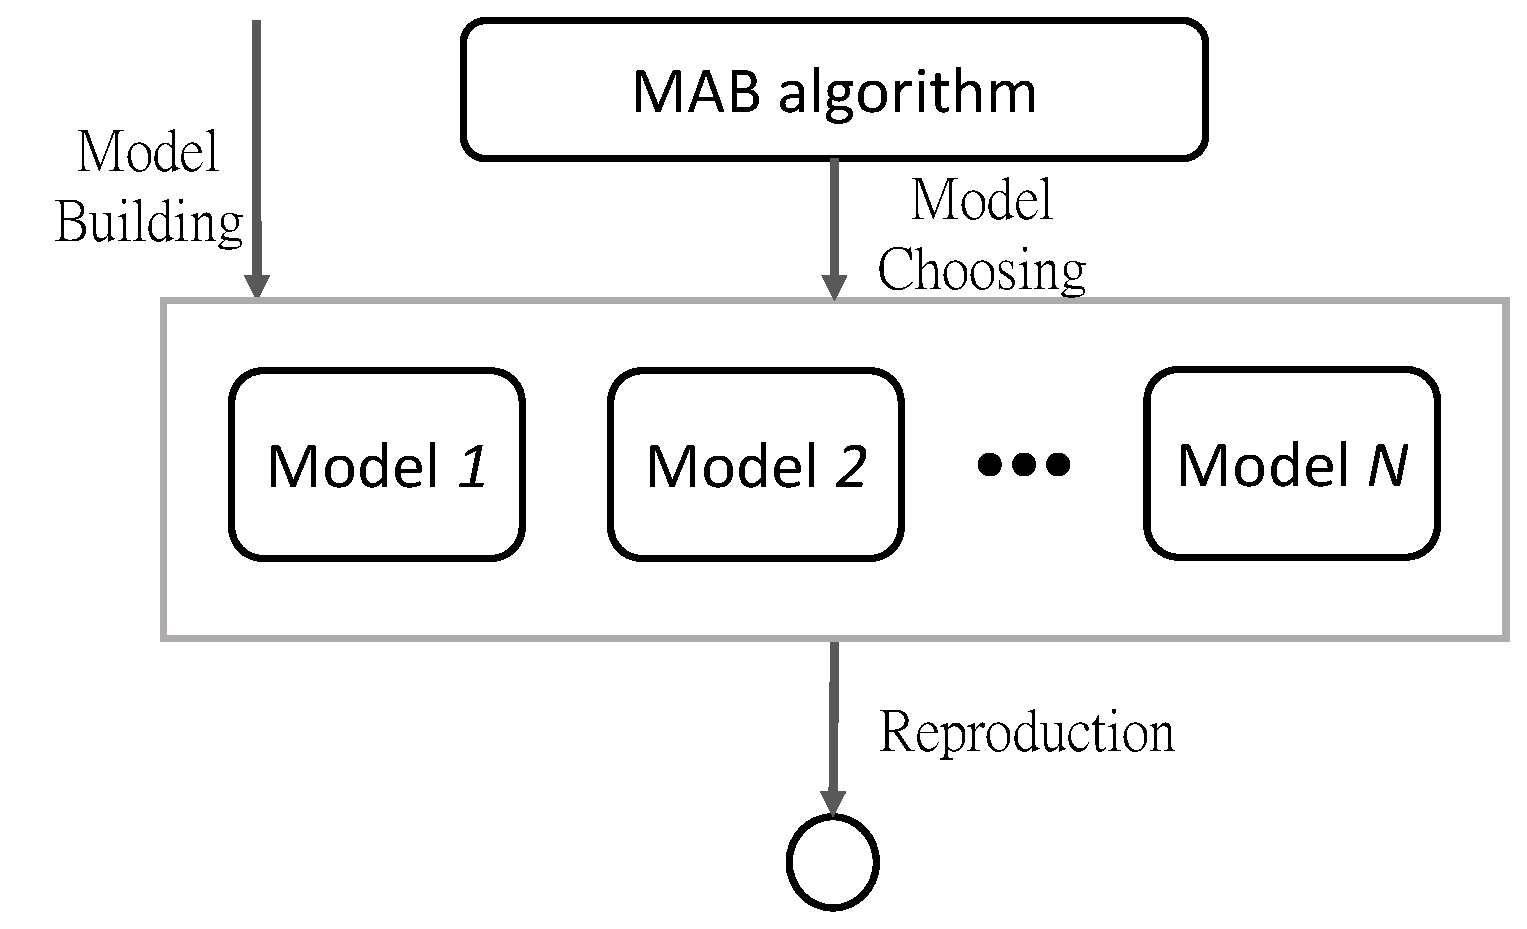
\includegraphics[width=0.8\textwidth]{model_adaptation_flow.eps}
    \caption{The Model Adaptation Flow}
    \label{fig:model_adaptation_flow}
\end{figure}
In this paper, the model adaptation framework incorporates with the UCB algorithms for a preliminary study. Although many other MAB techniques exist and show good performances~\citep{Kuleshov2000}, the UCB family is commonly used recent years, and is easy to be implemented. Figure \ref{fig:model_adaptation_flow} shows the flow of the model adaptation framework. Along with the original EDA framework, the model adaptation adds a new phase ``Model Choosing'' between phase ``Model Building'' and ``Sampling''. As can be seen, instead of generating a population of new individual with one model in the original version of sampling procedure, in our framework, new individuals are sampled one by one with different models. 
{\LinesNumbered
\begin{algorithm}[htbp]
\SetKwInOut{Input}{input}
    \SetKwInOut{Output}{output}

    \KwIn{The initial population $P$,\newline
    The semantic model set $\mathbb{M}$
    }
    \KwOut{The offspring population $O$}
        generate one individuals from each model\;
        
            %select population of promising solution $S$\;
            update each model $m \in \mathbb{M}$\;
                randomly chose $p \in P$\;
                choose a semantic model $m_{UCB}$ with \textit{highest UCB value}\;
                
                let $p$ be the template, generate a new individual $c$ by model $m_{UCB}$\;
                \If{$c$ is better than $p$}{ 
                    $O \leftarrow P \cup \{c\} - \{p\}$\; 
                    reward model $m_j$ with value $1.0$\;
                } 
                \Else{
                    $O \leftarrow P$; \newline 
                    reward model $m_j$ with value $0.0$\;
                }
                
   
        return $O$\;
    \caption{Multi-armed Bandit Based Model Adaptation}
    \label{alg:model_adaptation}
\end{algorithm}}


Algorithm \ref{alg:model_adaptation} introduces a details pseudo-code of the proposed multi-armed bandit based model adaptation (MABMA). Lines 10 and 11 replace $p$ with the newly generated individual $c$. To improve performance, we will introduce a new methodology to choose replaced individual in next chapter. As we treat the semantic models as arms in the MAB problem, at the initialization stage of the algorithm, the UCB algorithms needs initial value of the semantic models. Thus, each model $m_j$ have to generate one new individual by a randomly picked template for the initialization of UCB.

% Toward Comparison-based Adaptive Operator Selection
Properly rewarding the selected arm is a crucial element that should be carefully designed to ensure success~\citep{fialho2010analyzing}. The choice of the reward must encourage exploitation of the best arm while still allowing exploration of the other arms. Most methods use as raw reward the fitness improvement of the newborn offspring compared to a base individual, that might be its parent~\citep{barbosa2000adaptive, fialho2008extreme, fialho2009analysis, lobo1997decision, tuson1998adapting}, the current best in the population~\citep{Davis:1989:AOP:93126.93146}, or the median individual of the current population~\citep{Julstrom:1995:YDM:645514.657934}. The concept used in our case is borrowed from an assumption made in original UCB~\citep{Auer2002} -- the reward are with support in $[0,1]$. The reward given to the bandit is binary. An arm is assigned a reward of $1$ if the fitness of the newborn individual is better than the template, and 0 otherwise. 

%Sustainable Cooperative Coevolution with a Multi-Armed Bandit
This reward policy shares similar arguments with the policy used in~\citep{DeRainville:2013:SCC:2463372.2463556}. The direct fitness allocation suffers when the bandit is updated with a new fitness causing a loss -- if this fitness dominates any other arm causing a gain, the arm receives a higher credit for the loss. Since the template plays a critical role in the fitness of the new born individual, the fitness cannot reflect the appropriateness of a semantic model. Furthermore, the scale of the fitness value dramatically differs from problem to problem, or even from instance to instance. The fitness can not reflect the difference between two permutations. For instance, two permutation could have huge difference in the fitness because merely two nodes swapped its position in the permutation.


\subsection{Empirical Study}

In this subsection, the performance of MABMA is investigated. Several permutation problems are tested. For comparison, MABMA with  UCB1 and UCB1-Tuned are be tested. In the experiment of Multi-armed Bandit Based Model Adaptation,  EHM, NHM and the PL model are used. For each instance, we perform independent 10 runs with the population size $N = 2 \times L$ and the NFE limit $E_{max} = L \times 40000$. In this section, CVRP and the variation of CVRP -- the vehicle routing problem with Time Window (VRPTW)~\citep{toth2001vehicle} -- are tested.

%The experiment settings are as follows:
%\begin{itemize}
    %\item repeat 10 times,
    %\item the NHM, the EHM  and the PL model are used,
    %\item population size $N=1000$ for TSP and $N=100$ for the flat problem,
    %\item the bias ratio $B_{ratio} = 0.0000$,
    %\item template technique is used,
    %\item the cut-point number is 3 for template.
%\end{itemize}

\begin{table}[t]
    \centering
    \begin{tabular}{|l|l|l|l|l|l|}
    \hline
    \textbf{} & \textbf{EHBSA}       & \textbf{MABMA-UCB1} & \textbf{MABMA-UCBT} & \textbf{NHBSA} & \textbf{PLEDA} \\ \hline
    \textbf{A-n32-k5} & 1            & 5                  & 3              & 2           & 4         \\ \hline
    \textbf{A-n33-k5} & 1.5          & 4                  & 1.5            & 3           & 5         \\ \hline
    \textbf{A-n33-k6} & 1.5          & 1.5                & 3              & 4           & 5         \\ \hline
    \textbf{A-n34-k5} & 1            & 2                  & 3              & 4           & 5         \\ \hline
    \textbf{A-n36-k5} & 1            & 4                  & 2              & 3           & 5         \\ \hline
    \textbf{A-n63-k9} & 2            & 3                  & 1              & 4           & 5         \\ \hline
    \textbf{A-n64-k9} & 1            & 2                  & 3              & 4           & 5         \\ \hline
    \textbf{A-n65-k9} & 1            & 2                  & 3              & 4           & 5         \\ \hline
    \textbf{A-n69-k9} & 1            & 3                  & 2              & 4           & 5         \\ \hline
    \textbf{A-n80-k9} & 1            & 3                  & 2              & 4           & 5         \\ \hline
    \end{tabular} 
    \caption{The rank on CVRP}
    \label{tb:mabma_result}
\end{table}

\begin{table}[t]
    \centering
        \begin{tabular}{|l|l|l|l|l|l|}
        \hline
        \textbf{} & \textbf{EHBSA}       & \textbf{MABMA-UCB1} & \textbf{MABMA-UCBT} & \textbf{NHBSA} & \textbf{PLEDA} \\ \hline
        \textbf{C101\_0025}  & 2                  & 2                   & 2              & 4           & 5         \\ \hline
        \textbf{C103\_0025}  & 2                  & 2                   & 2              & 4           & 5         \\ \hline
        \textbf{RC102\_0025} & 1                  & 2                   & 3              & 5           & 4         \\ \hline
        \textbf{RC105\_0050} & 3                  & 2                   & 1              & 4           & 5         \\ \hline
        \textbf{C101\_0100}  & 4                  & 1                   & 2              & 3           & 5         \\ \hline
        \textbf{C101\_0025}  & 3                  & 1.5                 & 1.5            & 4           & 5         \\ \hline
        \textbf{C103\_0025}  & 3                  & 1.5                 & 1.5            & 4           & 5         \\ \hline
        \textbf{RC102\_0025} & 1                  & 2                   & 3              & 5           & 4         \\ \hline
        \textbf{RC105\_0050} & 3                  & 2                   & 1              & 4           & 5         \\ \hline
        \textbf{C101\_0100}  & 4                  & 1                   & 2              & 3           & 5         \\ \hline
        \end{tabular}
    \caption{The rank of the fvVRPTW}
    \label{tb:mabma_result}
\end{table}

    


The results are shown in Table \ref{tb:mabma_result}. MABMA-UCB1 is for MABMA with the UCB1 algorithm; MABMA-UCBT is for MABMA with the UCB1-Tuned algorithm. The values listed in the tables are the average of the best fitness of the algorithm obtained in 10 trials. Because CVRP aims to minimize the distance vehicles traveled, the fitness is the smaller, the better the performance. 

In CVRP instances, EHBSA outperforms the other algorithms. As can be seen, the average fitnesses of the MABMA algorithms are most close to the ones of optimal model, EHM. As the problem size becomes larger, the difference between EHBSA and MABMA decreases. In the fvVRPTW, MABMAs outperform the other algorithms on large problem instances. On the easier problem instance, MABMAs and EHBSA has identically performance, because they achieve the optimal solution.

Remarkably, on CVRP, the performance of MABMA-UCBT is more closer to that of EHBSA than that of MABMA-UCB1, while MABMA-UCB1 achieve better performance in the fvVRPTW. This fact may be caused by the variance factor in the UCB1-Tuned algorithm can help the MABMA stick to the most appropriate model better. However, when the most appropriate model is not existed, the UCB1 algorithm can start to explore in the earlier stage.


